\documentclass[class={IEEEtran}]{standalone}
\usepackage{tikz}

\pagestyle{empty}
\usetikzlibrary{shapes.geometric,shapes.arrows,positioning,calc,arrows.meta,math}

\tikzset{ARROW/.style={thick, -stealth}}
\tikzset{ORACLE/.style={rectangle, minimum width=9.3em, minimum height=10.5ex, draw, semithick, align=flush left, anchor=north east}}

\linespread{1.25}

\begin{document}
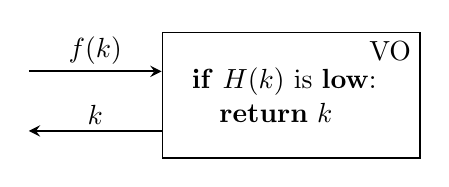
\begin{tikzpicture}
    \node[ORACLE] (n_oracle) {
        \hspace{-0.5em}\textbf{if} $H(k)$ is \textbf{low}: \\
        \hspace{0.5em}\textbf{return} $k$
    };
    \node[anchor=north east] at (n_oracle.north east) {VO};

    \coordinate (input1) at ($(n_oracle.west)+(-4.8em, 2ex)$);
    \coordinate (input1_end) at ($(input1-|n_oracle.west)$);
    \draw[ARROW] (input1) -- (input1_end) node[midway,above=-0.3ex]{$f(k)$};


    \coordinate (output) at ($(n_oracle.west)+(-4.8em, -3ex)$);
    \coordinate (output_end) at ($(output-|n_oracle.west)$);
    \draw[ARROW] (output_end) -- (output) node[midway,above=-0.3ex]{$k$};
\end{tikzpicture}
\end{document}
